\documentclass[a4paper,spanish]{exam}
\usepackage[spanish]{babel}
%\usepackage[utf8]{inputenc}
\usepackage{multicol}
%\usepackage[latin1]{inputenc}
\usepackage{fontspec}%la posta para las tildes con lualatex
\usepackage[margin=0.5in]{geometry}
\usepackage{amsmath,amssymb}
\usepackage{multicol}
\usepackage{natbib}
\usepackage{graphicx}
\usepackage{hyperref}
\usepackage{epstopdf}
\usepackage{capt-of}
\usepackage[space]{grffile}
\usepackage[usenames]{color}
%los de aca abajo capaz no los uso
\newcommand{\class}{Matemática: Evaluación de Funciones Racionales {\tiny (Recuperatorio)}}
\newcommand{\term}{2° Trimestre 2015}
\newcommand{\examnum}{Tema 4}
\newcommand{\examprof}{Alexis Gomel}
\newcommand{\examdate}{15/9/2015}
\newcommand{\timelimit}{60 Minutes}%no lo uso
\newcommand{\Ts}{\rule{0pt}{2.8ex}}       % Top strut
\newcommand{\Bs}{\rule[-1.5ex]{0pt}{0pt}} % Bottom strut
%el header de las hojas.
\pagestyle{head}
\firstpageheader{}{}{}
\runningheader{\class}{\examnum\ - pagina \thepage\ de \numpages}{\examdate}
\runningheadrule


\begin{document}
\noindent
\begin{minipage}{0.92\linewidth}
	\begin{tabular*}{\textwidth}{l @{\extracolsep{\fill}} r @{\extracolsep{6pt}} l}
		\textbf{\class} & \textbf{Profesor: \examprof}\\
		\textbf{\examnum}  & \textbf{}   \\
		%& Teaching Assistant & \makebox[2in]{\hrulefill}
		\textbf{Nombre: } \makebox[2in]{\hrulefill} & \textbf{\examdate} 
	\end{tabular*}\\
\end{minipage}
\begin{minipage}[r]{0.08\linewidth}
	\begin{flushright}
		
\includegraphics[width=\linewidth]{bost.png}
	\end{flushright}
\end{minipage}\\
\rule[2ex]{\textwidth}{2pt}

%%%%%%%%%%%%%%%%%%%%%%%%%%%%%%%%%%%%%%%%%%%

\begin{center}
	\textsl{\textbf{\underline{Justificar}}} cada respuesta. El trabajo practico se entrega \textbf{\underline{escrito en tinta}}.\\
	Si se traban con un ejercicio sigan con el siguiente.
	\textbf{Preguntas:} $\bigcirc \bigcirc \bigcirc  \bigcirc $
\end{center}

\begin{table}[h]
\centering
%\caption{My caption}
\label{my-label}
\begin{tabular}{|l|c|c|c|c|}
\hline
Ejercicio        & 1 & 2 & 3 & Nota \\ \hline
Puntaje máximo   & 4 & 2 & 4 &   10   \\ \hline
Puntaje obtenido &   &   &   &      \\ \hline
\end{tabular}
\end{table}

Si se traban con algún ejercicio, pasen al siguiente y vuelvan a intentar mas tarde con el que dejaron.

\begin{enumerate}

%uno de inversa


%homografica
\item Graficar la función homografica \[ y=\frac{5}{x+1}-1 \] especificando el Dominio, la Imagen, las raíces y las asintotas. \\

Encontrar para que valores de $x$ la función es mayor o igual a $1$.

%una a graficar de las fdificiles

\item Cual función corresponde al gráfico. 
%aca va una tabla y unos graficos

\begin{minipage}{0.5\textwidth}
\centering
%\begin{table}[!h]
%\caption{mc1}
\label{mc1}
\begin{tabular}{|c|c|c|}
\hline
$\frac{10x^6}{(x+4)^2(x-4)^2}$  & $\frac{-10x^4}{(x^2+16)(x^2-16)}$ & $\frac{10x^4}{(x+4)^2(x-4)^2}$ \Ts \Bs   \\ \hline
   &   &      \\ \hline
\end{tabular}\\
%\end{table}
%\begin{figure}[h]
\centering
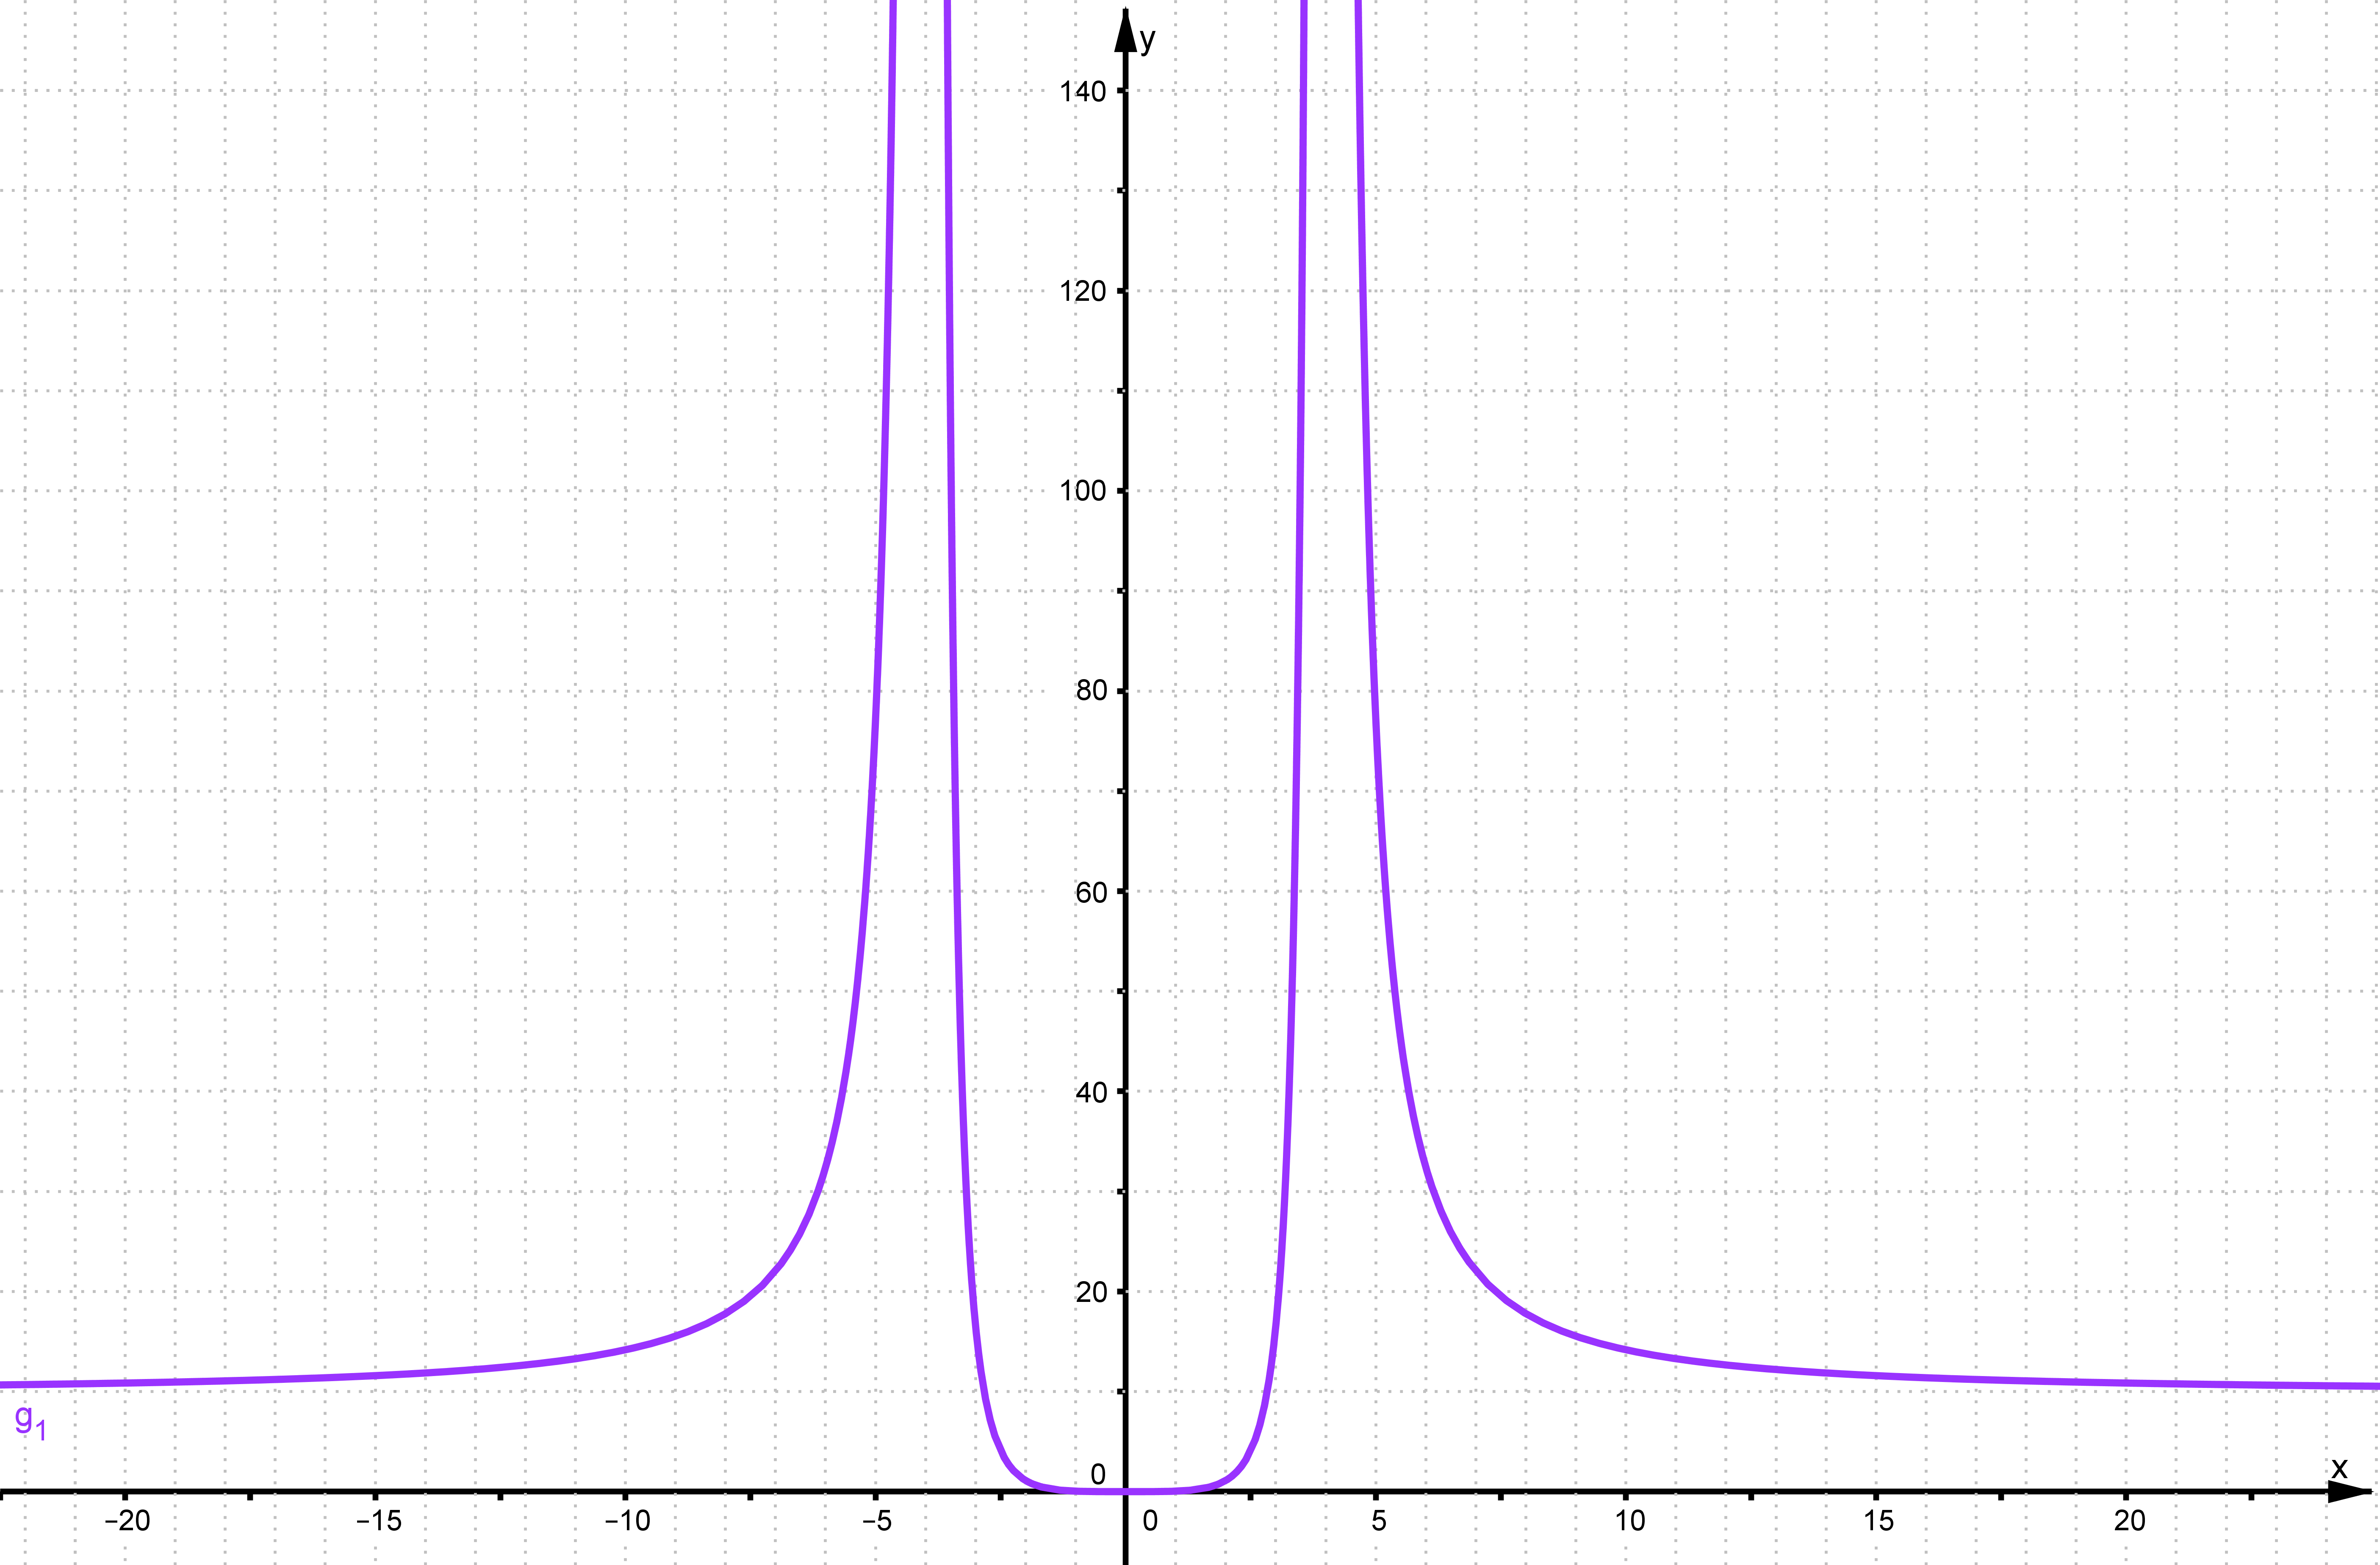
\includegraphics[width= 0.95\linewidth]{problematema11.png}
%\end{figure}
%graficos
\end{minipage}
\begin{minipage}{.5\textwidth}
\centering
%\begin{table}[!h]
%\caption{mc1}
%\label{mc1}
\begin{tabular}{|c|c|c|}
\hline
$\frac{x^5}{15(x+20)(x-20)}$  & $\frac{x^5}{15(x+20)(x-20)(x-10)}$ & $\frac{x^2}{15(x+20)(x-20)(x-10)}$ \Ts \Bs   \\ \hline
   &   &      \\ \hline
\end{tabular}\\
%\end{table}
%\begin{figure}[h]
\centering
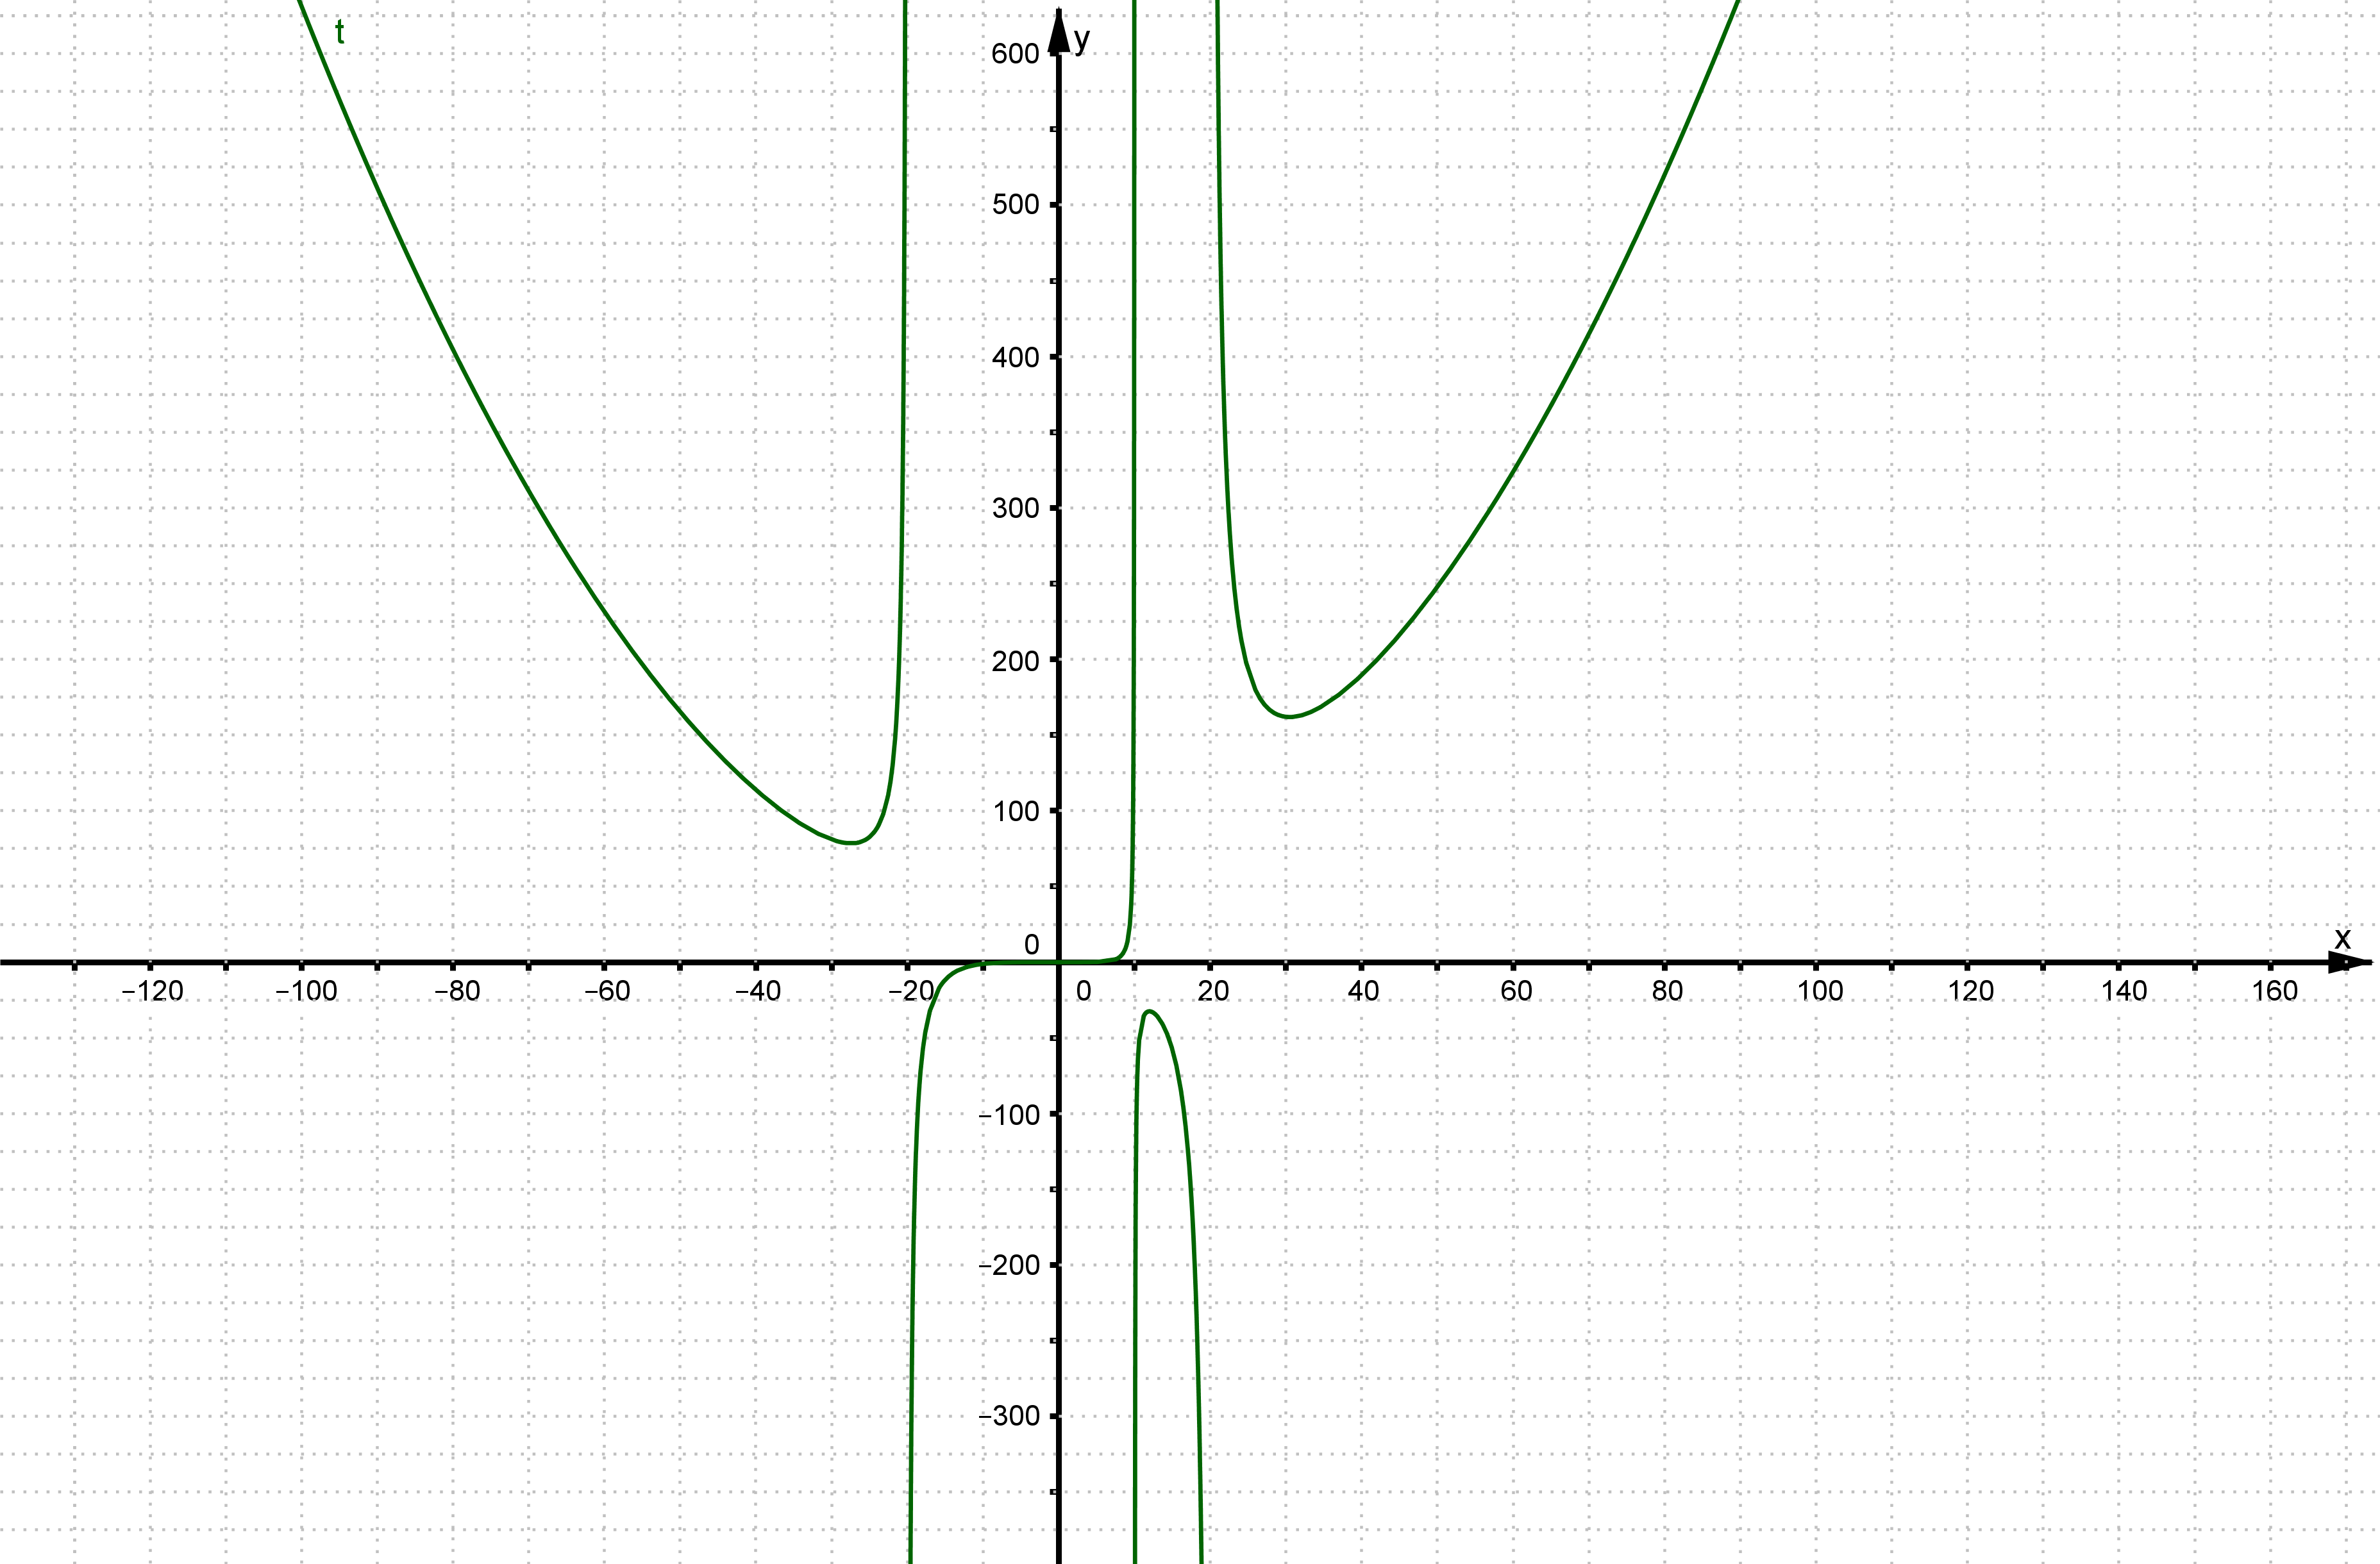
\includegraphics[width= 0.95\linewidth]{problematemarec13.png}
%\end{figure}
\end{minipage}


\item  Graficar la función \[ y=\frac{5(x+4)(x-4)}{x^2}  \]. Indicando el Dominio, la Imagen, las raíces y las asintotas.

 \item (bonus)\textbf{Extra:}
 Si ya terminaste los demás, este ejercicio sirve como un bonus para darte un empujón si estas cerca de aprobar, o para redondear la nota para arriba.\\
 
Demostrar que la multiplicación por una función racional y la potenciación (para potencias pertenecientes a los enteros) de una función racional $f(x)=\frac{P(x)}{Q(x)}$ da como resultado una función racional. ¿Porque necesito restringirme a los enteros?.

Es decir que $h(x)=f(x).g(x)$ también es una función racional (si $f$ y $g$ son funciones racionales), sin importar los grados de los polinomios de $P,Q,L$ y $M$; y $(f(x))^{n}$ también lo es. 

\end{enumerate}
 
\rule[2ex]{\textwidth}{2pt}
 
"There’s as many atoms in a single molecule of your DNA as there are stars in the typical galaxy. We are, each of us, a little universe."
$―$ Neil deGrasse Tyson, Cosmos 

%\newpage

%\section*{Respuestas}

%1: a)3 b)49 c)-3 d)$ 1/16$ e)2 f)$ 1+0,68 $ g)$ 1,46$ h)$2.0,68$ 

%2: a)27 b)2  c)2 d)6 %d)$\frac{5}{3.c^2}$

%3: 1.
%\begin{figure}[h!]
%\centering
%\includegraphics[width=0.7\textwidth]{encontrarlog2xmenos2.jpg}
%\caption{}
%\label{fig:logaritmo}
%\end{figure}

%3: 2.$log_2(x-2)$



\end{document}
